\chapter{Chromatin immunoprecepitation}

\section{Intro}
Chromatin immunoprecipitation followed by sequencing, also known as ChIP-sequencing or ChIP-seq, is a modern and relatively cheap method to analyze any protein associated with DNA. 
The most frequently investigated chromatin-associated proteins are transcription factors (TF), modifies histones, components of the transcriptional machinery, and chromatin-modifying enzymes.
Advances in high-throughput parallel sequencing technology and computational methods enable generate and analyze extremely large data sets. 
Unlike ChIP-on-chip, ChIP-seq was developed to understand genome-wide profiling and does not rely on knowledge of exact binding loci.~\cite{park2009chip} .


\section{Experiment design}

A typical protocol has many steps. 
The consideration od the first step depends on the properties of the protein under investigation. 
For example, histone-DNA interactions are strong enough. 
Thus the fixation using formaldehyde as a crosslinking agent may not be necessary~\cite{barski2008identification}. 
On the other hand, proteins associated with DNA for a short time require a crosslinking step. 
In the case of histone deacetylases (HDACs) and histone acetyltransferases (HATs), an additional disuccinimidyl glutarate (DSG) treatment step before formaldehyde crosslinking demands~\cite{wang2009genome}. 

Cross-linked chromatin is fragmented before ChIP. 
Fragmentation way is depending on the purpose of the experiment, cell type, number of cells, fixation conditions. 
For nucleosome modifications, MNase digestion may be preferred~\cite{kidder2011chip}.  
The method allows generating high-resolution data of mononucleosome sized particles. 
However, the nucleosome instability may cause the loss of signal.
To identify TF binding events, sonication of crosslinked chromatin is a preferable method. 
In this case, the micrococcal nuclease may cause degradation of the linker DNA~\cite{kidder2011chip}.
The sonication conditions should be optimized for each experiment type. 
A Sonication buffer can influence the result~\cite{steger2008dot1l}. 
It is also important to avoid oversonication during the library preparation for transcription factors. 

The successful ChIP experiment depends on the isolation of the protein under study from a complex mixture of the chromatin fragments and associated proteins. 
The specific antibody against a protein of interest is using during the immunoprecipitation step. 
This procedure allows the removal of non-specific binding sites. 
The right choice of antibody is an essential factor for the ChIP-seq experiment. 
Many experiments are orienting on newly discovered proteins. 
And in these cases, specific antibodies are not available, and epitope-tagged methods can be useful~\cite{brizzard2008epitope, goldberg2010distinct}.

\section{Library construction, sequencing and mapping}

After chromatin purification with and without immunoprecipitation to prepare ChIP and corresponding input DNA fragments, the material is ready to be sequenced. 
The size range of 150 to 300 bp fragment length selection is equivalent to mono- and dinucleosome chromatin fragments~\cite{kidder2011chip}.

The goal of the ChIP-sequencing is to obtain reads long enough to map uniquely to the reference.  
In many cases, 36-50 bp will be enough even for a complex organism such as a human. 
The longer reads sequenced, the deeper coverage per base may be achieved.
Libraries can be sequenced using a single-end or paired-end strategy. 
Paired-end sequencing can be useful to increase sequencing coverage, improve alignment efficiency into repetitive regions, and detect fragment size~\cite{kidder2011chip, chen2012systematic}.


\begin{figure}[b!]
\centering
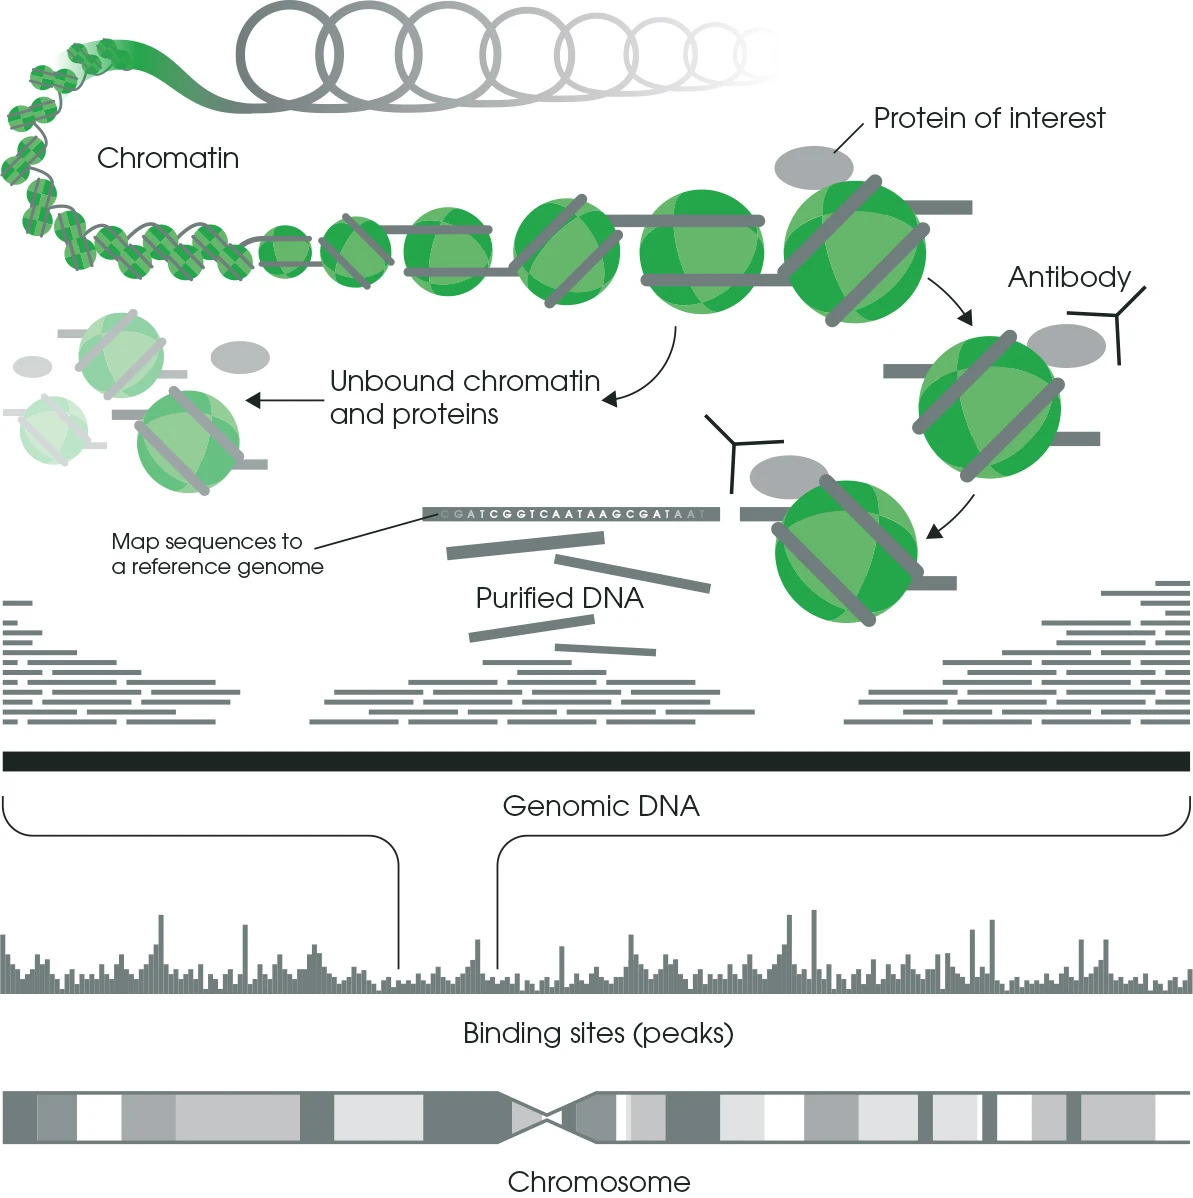
\includegraphics[width=\textwidth]{../img/chip.jpeg}
\captionsource{Overview of ChIP-seq experiment.}{www.abcam.com}
\label{fig:graph_classes}
\end{figure}

Next-generation sequencing technological advancements have facilitated the production of a huge amount of sequencing data. 
Multiple barcoded ChIP-seq libraries pooled together and sequenced in a single lane~\cite{craig2008identification} to reduce the cost of the experiment and produce high-quality data.
There are several sequencing technologies available. The big amount of data is generating through the Illumina platform, which produces about 100-400 million reads per run.

Row data of short sequenced tags often appear in fastq format containing sequence information and quality scores. Such files may contain 10 to 60 million reads. Several alignment tools have been developed based on extended Burrows-Wheeler transform (BWT)~\cite{li2009fast, siren2014indexing}.
Unlike RNA-seq with exon junctions, the ChIP-seq experiment does not require to find spliced alignment. 
Uniquely mapped reads with minimal allowed mismatches are sufficient to analyze typical TF and also simplify further analysis. 
However, allowing the random location for multiple mapped reads may increase the sensitivity of peak detection. 
The ration of the unique mapped reads over the total number of mapped reads is one of the parameters of the library quality assessment and should not be below 50\%~\cite{shin2013computational}.
